\chapter{Jednoparametrové modely}

\section{Odhad pravděpodobnosti z binomických dat}

V binomickém modelu odhadujeme neznámou pravděpodobnost úspěchu v populaci na základě výsledků posloupnosti Bernoulliho pokusů. Připomeňme, že výsledek pozorování v rámci Bernoulliho pokusu může nabývat pouze dvou stavů - úspěchu a neúspěchu. Ze základů statistiky víme, že binomický model je definován jako
\begin{equation}
p(y|\theta) = \textit{Bin}(y|n, \theta) = {n \choose y} \theta^y (1 - \theta)^{n - y},
\end{equation}
kde $n$ představuje celkový počet pokusů, $y$ celkový počet úspěchů a $\theta$ hledanou pravděpodobnost úspěchu v populaci. 

\subsection{Ilustrativní příklad - odhad pravděpodobnosti odhadu narození ženy}

V následujícím textu vysvětlíme binomický model na ilustrativním příkladu odhadu pravděpodobnosti narození ženy.

\subsubsection{Aposteriorní rozdělení}

Předpokládejme, že počet všech narozených dětí je $n$, z čehož je $y$ ženského pohlaví. Nejprve je třeba zvolit apriorní rozdělení parametru $\theta$, které vyjadřuje podíl žen na celkovém počtu narozených dětí pro danou populaci. Jestliže má apriorní rozdělení parametru $\theta$ charakter uniformního rozdělení nad intervalem $[0, 1]$, lze aplikací Bayesova pravidla (1.3) na (2.1) odvodit aposteriorní rozdělení parametru $\theta$ jako 
\begin{equation}
\begin{split}
Pr(\theta \in (\theta_1, \theta_2) | y) & = \frac{Pr(\theta \in (\theta_1, \theta_2), y)}{p(y)}\\
 & = \frac{\int_{\theta_1}^{\theta_2} p(y|\theta)p(\theta)d\theta}{p(y)}\\
 & = \frac{\int_{\theta_1}^{\theta_2} {n \choose y} \theta^y (1 - \theta) ^ {n - y}d \theta}{p(y)}.
\end{split}
\end{equation}
Lze dokázat, že jmenovatel (2.2) je možné upravit do tvaru
\begin{equation}
\begin{split}
p(y) &= \int_0^1 {n \choose y} \theta^y (1 - \theta)^{n - y}d\theta\\
 & = \frac{1}{n + 1} \quad y = 0, ..., n.
\end{split}
\end{equation}
Tento výsledek nám říká, že apriori jsou všechny hodnoty $y$ stejně pravděpodobné. Čitatel (2.2) představuje nekompletní beta integrál, který nemá analytické řešení pro velká $y$ a $n - y$.

Výsledné aposteriorní rozdělení má podobu
\begin{equation}
p(\theta | y) = \frac{{n \choose y}}{n + 1} \theta^y (1 - \theta) ^ {n - y} d\theta.
\end{equation}
Pro fixní hodnoty $n$ a $y$ není $\frac{{n \choose y}}{n + 1}$ funkcí neznámého parametru $\theta$. Aposteriorní rozdělení parametru $\theta$ tak můžeme chápat jako nenormalizované beta rozdělení, tj.
\begin{equation}
p(\theta | y) \varpropto \theta^y (1 - \theta)^{n - y}.
\end{equation}
Vztah (2.5) nám pro zvolené $n$ a $y$ umožňuje grafickou prezentaci aposteriorního rozdělení, viz. obrázek 2.1.
\begin{figure}[htp]
\centering
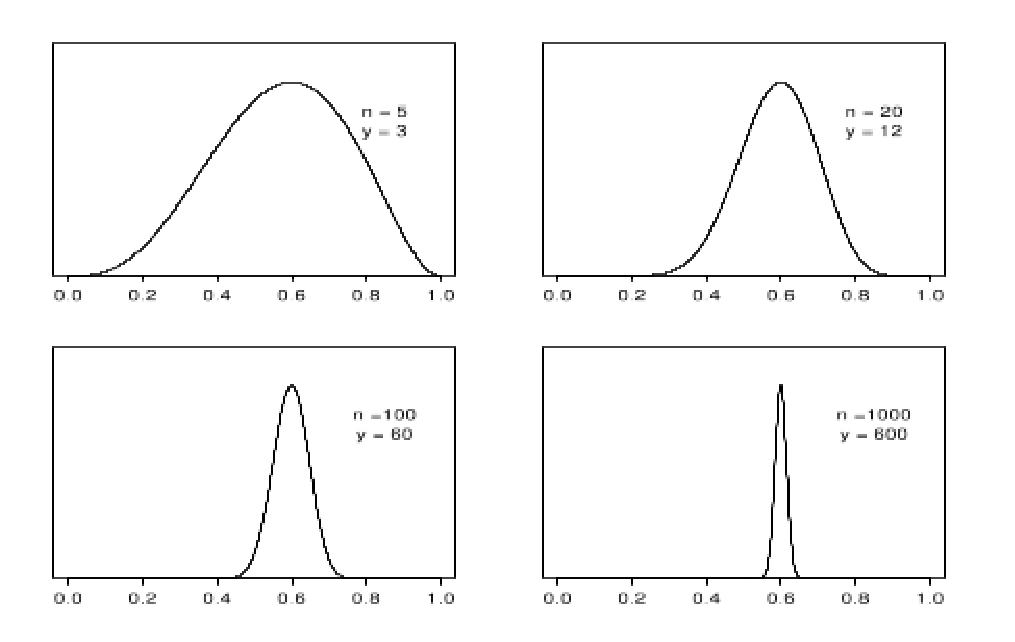
\includegraphics[scale = 0.65]{pictures/fig_2_1.eps}
\caption{Nenormalizované aposteriorní rozdělení parametru $\theta$ pro vybrané hodnoty $n$ a $y$ za předpokladu apriorního uniformního rozdělení parametru $\theta$.}
\label{fig_2_1}
\end{figure}

\subsubsection{Aposteriorní predikce}

Apriorní prediktivní rozdělení lze vyjádřit analyticky pomocí (2.3). Tato pravděpodobnost říká, že libovolná hodnota $y$ z intervalu nula až $n$ má pravděpodobnost $\frac{1}{n + 1}$, což je logický důsledek našeho apriorního předpokladu o uniformním rozdělení parametru $\theta$.

Aposteriorní prediktivní rozdělení zohledňuje výsledek dodatečných Bernouliho pokusů. Pro zjednodušení předpokládejme pouze jeden dodatečný pokus, jehož výsledek označme $\tilde{y}$. Platí
\begin{equation}
\begin{split}
Pr(\tilde{y} = 1 | y) & = \int_0^1 Pr(\tilde{y} = 1 | \theta, y)p(\theta|y)d\theta\\
 & = \int_0^1 \theta \cdot p(\theta | y) d\theta = E(\theta | y) = \frac{y + 1}{n + 2},
\end{split}
\end{equation}
což vyplývá z vlastností beta rozdělení. Tento výsledek, založený na předpokladu apriorního uniformního rozdělení, je známý jako Laplacův zákon posloupnosti (Laplace's law of succession).

\subsubsection{Historická vsuvka}

Již před dvěma stoletími dokázal Laplace, že pravděpodobnost narození ženy je menší než 50.00\%. Při řešení problémů aplikoval binomický model doplněný o předpoklad apriorního uniformního rozdělení parametru $\theta$, který představoval pravděpodobnost narození ženy. V Paříži se letech 1745 až 1770 se narodilo 241~945 dětí ženského a 251~527 dětí mužského pohlaví. Na základě těchto pozorování Laplace dokázal, že
\begin{equation*}
Pr(\theta \ge 0.50 | y = 241~945, n = 241~945 + 251~527) \approx 1.15 \cdot 10^{-42},
\end{equation*}
což mu dávalo právo tvrdit, že hodnota parametru $\theta$ je menší než 0.50.

\section{Aposteriorní pravděpodobnost jako kompromis mezi daty a apriorní informací}

Proces Bayesovské inference zahrnuje přechod od apriorního rozdělení $p(\theta)$ k aposteriornímu rozdělení $p(\theta | y)$. Je tak přirozené očekávat, že mezi těmito dvěma rozděleními mohou existovat určité vazby.

Na jednu z těchto vazeb jsme již narazili ve vztazích (1.11) a (1.13), kdy výměnou $(u, v)$ za $(\theta, y)$ získáváme
\begin{equation}
E(\theta) = E(E(\theta | y))
\end{equation}
a
\begin{equation}
var(\theta) = E(var(\theta | y)) + var(E(\theta | y)).
\end{equation}

Připomeňme, že apriorní střední hodnota parametru $\theta$ je průměrem aposteriorních středních hodnot přes všechna možná data. Aposteriorní rozptyl parametru $\theta$ je pak v průměru menší než apriorní rozptyl, kdy výše rozdílu závisí na druhém členu pravé strany rovnice (2.8), tj. na rozptylu aposteriorních středních hodnot přes všechna možná data. Čím vyšší je rozptyl těchto aposteriorních středních hodnot, tím vyšší je potenciál redukce nejistoty parametru $\theta$. Je nutné si však uvědomit, že vztahy (2.7) a (2.8) popisují pouze očekávané hodnoty a že v některých situacích může být aposteriorní rozptyl i vyšší než apriorní rozptyl.

Pro výše uvedený příklad binomického modelu s apriorním uniformním rozdělením parametru $\theta$ platí, že apriorní střední hodnota $E(\theta)$ je rovna $\frac{1}{2}$. Aposteriorní střední hodnota $\frac{y + 1}{n + 2}$ je pak kompromisem mezi apriorní střední hodnotou $\frac{1}{2}$ a výběrovou střední hodnotou $\frac{y}{n}$. Toto je obecná vlastnost Bayesovské inference - aposteriorní rozdělení je centrované na bodě, který představuje kompromis mezi apriorním rozdělením a pozorovanými daty, přičemž role dat vzrůstá s jejich objemem.

\section{Charakteristiky aposteriorního rozdělení}

Aposteriorní rozdělení $p(\theta | y)$ je vhodné graficky znázornit tak, jak jsme učinili na obrázku 2.1. V řadě praktických případů je graf aposteriorního rozdělení žádoucí doplnit o numerické statistiky jako jsou střední hodnota, medián, modus či směrodatná odchylka. Nejistotu aposteriorního rozdělení lze popsat pomocí kvantilů a rozpětím mezi těmito kvantily. Pouze v omezeném počtu případů je možné kvantily a jejich rozpětí vyjádřit analyticky. Vždy je však možné je vypočíst metodou Monte-Carlo.

\section{Informativní apriorní rozdělení}

Apriorní rozdělení lze interpretovat dvěma způsoby. Můžeme ho chápat jako rozdělení, které charakterizuje populaci možných hodnot parametru $\theta$, z nichž je pak parametr náhodně vybrán. Nebo ho můžeme chápat jako rozdělení, které odráží všechny naše znalosti a předpoklady týkající se parametru $\theta$, přičemž hodnotu tohoto parametru chápeme jako náhodnou realizaci z apriorního rozdělení.

Apriorní rozdělení by mělo zahrnovat všechny přijatelné hodnoty parametru $\theta$, však nemusí být nezbytně koncentrováno kolem skutečné hodnoty. Často se totiž stává, že informace o $\theta$ obsažená v datech převáží jakoukoliv rozumnou specifikaci apriorního rozdělení. S tímto přístupem jsme se setkali už v předchozím textu, kdy jsme uvažovali apriorní uniformní rozdělení parametru $\theta$ na intervalu $[0, 1]$, ačkoliv bychom pravděpodobně mohli uvažovat mnohem užší interval.

\subsection{Binomický model s alternativním apriorním rozdělením}

\subsubsection{Apriorní beta rozdělení}

Předpokládejme, že věrohodností funkce (2.1), kterou lze chápat jako funkci parametru $\theta$, má tvar
\begin{equation}
p(y|\theta) \varpropto \theta^y (1 - \theta)^{n - y}.
\end{equation}
Jedná se tedy o beta rozdělení $y | \theta \sim \textit{Beta}(y - 1, n - y - 1)$. Pokud má apriorní rozdělení stejnou formu, tj.
\begin{equation}
p(\theta) \varpropto \theta^{\alpha - 1}(1 - \theta)^{\beta - 1},
\end{equation}
pak má aposteriorní rozdělení taktéž shodnou formu.

Předpokládejme, že máme k dispozici rozumné hodnoty parametrů $\alpha$ a $\beta$. Aposteriorní rozdělení je pak definováno jako
\begin{equation}
\begin{split}
p(\theta | y) & \varpropto \theta^y (1 - \theta)^{n - y} \theta^{\alpha - 1}(1 - \theta)^{\beta - 1}\\
 & = \theta^{y + \alpha - 1} (1 - \theta)^{n - y + \beta - 1}\\
 & = \textit{Beta}(\theta | \alpha + y, \beta + n - y)
\end{split}
\end{equation}

Jestliže má aposteriorní rozdělení stejnou parametrickou formu jako apriorní rozdělení, hovoříme o tzv. konjugaci (conjugacy).

Aposteriorní střední hodnota parametru $\theta$ má tvar
\begin{equation}
E(\theta | y) = \frac{\alpha + y}{\alpha + \beta + n}
\end{equation}
a nachází se tak vždy mezi výběrovým podílem $\frac{y}{n}$ a apriorní střední hodnotou $\frac{\alpha}{\alpha + \beta}$. Aposteriorní rozptyl je dán
\begin{equation}
var(\theta | y) = \frac{(\alpha + y)(\beta + n -y)}{(\alpha + \beta + n)^2(\alpha + \beta + n + 1)} = \frac{E(\theta|y)[1 - E(\theta | y)]}{\alpha + \beta + n + 1}.
\end{equation}
Pro fixní $\alpha$ a $\beta$ a vysoké $y$ a $n - y$ platí $E(\theta | y) \approx \frac{y}{n}$ a $var(\theta | y) \approx \frac{1}{n}\frac{y}{n}(1 - \frac{y}{n})$, přičemž $var(\theta | y)$ blíží nule rychlostí $\frac{1}{n}$. Limitně tak parametry apriorního rozdělení $\alpha$ a $\beta$ nemají vliv na podobu aposteriorního rozdělení.

\subsubsection{Apriorní normální rozdělení}

Pomocí centrální limitní věty zasazené do kontextu Bayesiánské statistiky lze dokázat
\begin{equation}
\Big(\frac{\theta - E(\theta | y)}{\sqrt{var(\theta | y)}} | y \Big) \rightarrow N(0, 1),
\end{equation}
což se často používá pro ospravedlnění aproximace aposteriorního rozdělení pomocí normálního rozdělení. V případě binomického parametru $\theta$ je aproximace pomocí normálního rozdělení přesnější, pokud použijeme transformaci $\ln(\theta \ (1 - \theta))$ namísto původního $\theta$. Touto transformací roztáhneme pravděpodobností prostor z $[0, 1]$ na $(-\infty, \infty)$, což je z pohledu normálního rozdělení vhodnější.

\subsection{Konjugátní apriorní rozdělení}

Jestliže $\mathcal{F}$ je třída výběrového rozdělení $p(y|\theta)$ a $\mathcal{P}$ je třída apriorního rozdělení parametru $\theta$, pak $\mathcal{P}$ je konjugát k $\mathcal{F}$, jestliže platí
\begin{equation}
p(\theta | y) \in \mathcal{P} \textit{ pro všechna } p(\cdot | \theta) \in \mathcal{F} \textit{ a } p(\cdot) \in \mathcal{P}.
\end{equation}
Výše uvedená definice je formálně vágní. Lze totiž vybrat $\mathcal{P}$ jako třídu všech rozdělení, což znamená, že $\mathcal{P}$ je vždy konjugát bez ohledu na výběrové rozdělení. My se však především zajímáme o tzv. přirozené konjugáty. Jedná se o případ, kdy $\mathcal{P}$ je množina všech rozdělení, které mají stejný funkcionální tvar jako věrohodnostní funkce.

\subsection{Nekonjugátní apriorní rozdělení}

Zásadní výhodou konjugátního apriorního rozdělení je snadná interpretace výsledků, které je často možné vyjádřit v analytické podobě, což značně usnadňuje navazující výpočty.

V praxi je často pro složitější modely nemožné nalézt vhodné konjugátní apriorní rozdělení. Ačkoliv je interpretace jejich aposteriorních inferencí méně transparentní a jejich výpočet je složitější, nepředstavují nekonjugátní apriorní rozdělení koncepční problém. V následujícím textu si představíme několik takovýchto příkladů.

\subsection{Konjugátní apriorní rozdělení, rodina exponenciálních pravděpodobnostních rozdělení a dostatečná statistika}

$\mathcal{F}$ je rodinou exponenciálních pravděpodobnostních rozdělení, pokud všechny její členy mají podobu
\begin{equation}
p(y_i | \theta) = f(y_i) g(\theta)e^{\phi(\theta)^T u(y_i)}.
\end{equation}
$\phi(\theta)$ a $u(y_i)$ jsou vektory se stejnou dimenzí jako $\theta$. Vektor $\phi(\theta)$ je nazýván přirozeným parametrem rodiny $\mathcal{F}$. Věrohodnostní funkce odpovídající posloupnosti $y = (y_1, ...,  y_n)$ nezávislých a identicky rozdělených pozorování má tvar
\begin{equation}
p(y | \theta) = \Big(\prod_{i = 1}^n f(y_1)\Big) g(\theta)^n e^{\Big( \phi(\theta)^T \sum_{i = 1}^n u(y_i)\Big)}.
\end{equation}
Pro dané $n$ a $y$ lze výše uvedený vztah chápat jako funkci parametru $\theta$, tj.
\begin{equation}
p(y | \theta) \varpropto g(\theta)^n e^{\phi(\theta)^T t(y)},
\end{equation}
kde $t(y) = \sum_{i = 1}^n u(y_i)$. $t(y)$ označujeme jako dostatečnou statistiku parametru $\theta$, protože věrohodnostní funkce parametru $\theta$ závisí na pozorováních $y$ pouze skrze $t(y)$. Pokud má apriorní rozdělení podobu
\begin{equation}
p(\theta) \varpropto g(\theta)^{\eta} e^{\phi(\theta)^T \nu},
\end{equation}
pak má aposteriorní rozdělení podobu
\begin{equation}
p(\theta | y) \varpropto g(\theta)^{\eta + n}e^{\phi(\theta)^T (\nu + t(y))},
\end{equation}
což mimo jiné dokazuje, že námi zvolené apriorní rozdělení je konjugát. Lze dokázat, že rodina exponenciálních pravděpodobnostních rozdělení je jedinou rodinou pravděpodobnostních rozdělení, které mají přirozené konjugátní apriorní rozdělení.

V předchozím textu jsme diskutovali binomické rozdělení s věrohodnostní funkcí $p(y|\theta, n) = \textit{Bin}(y| n, \theta)$, kde pro známé $n$ má konjugátní apriorní rozdělení parametru $\theta$ charakter beta rozdělení. Lze dokázat, že binomické rozdělení patří do rodiny exponenciálních rozdělení s přirozeným parametrem $logit(\theta)$.

\subsection{Ilustrativní příklad}

Jako specifický příklad faktoru, který může ovlivnit podíl narozených dětí ženského pohlaví, můžeme uvažovat tzv. placenta previa. Jedná se o situaci, kdy je během těhotenství placenta napojena v nižší části dělohy, což znemožňuje klasický porod. V Německu proběhla studie, která se na tuto problematiku zaměřovala. V jejím průběhu bylo zkoumáno 980 porodů, z nichž 437 připadalo na novorozence ženského pohlaví. Lze na základě těchto poznatků tvrdit, že v souvislosti s placenta previa je relativní podíl novorozenců ženského pohlaví nižší než je tomu v celkové populaci, tj. než 0.485?

\subsubsection{Apriorní uniformní rozdělení}

Za předpokladu apriorního uniformního rozdělení je aposteriorní pravděpodobnost narození jedince ženského pohlaví dána beta rozdělením $\textit{Beta}(438, 544)$. Aposteriorní střední hodnota a rozptyl parametru $\theta$ jsou tak 0.446 a 0.016. 95\% interval spolehlivosti je pak možné získat numerickou integrací beta rozdělení nebo aproximací pomocí normálního rozdělení. S přesností na tři desetinná místa se v obou případech jedná o interval $[0.414, 0.476]$.

Jak jsme však již zmínili dříve, v případě aproximace pravděpodobnostního rozdělení parametru $\theta$ pomocí normálního rozdělení je vhodnější použít logit transformaci.\footnote{Nejprve vygenerujeme z $\textit{Beta}(438,544)$ rozdělení tisíc náhodných pozorování, na které aplikujeme logit transformaci. Následně z transformovaných pozorování vypočteme střední hodnotu a rozptyl. Na základě odhadnuté střední hodnoty a rozptylu pak pomocí aproximace normálním rozdělením určíme požadovaný konfidenční interval. Nakonec tento konfidenční interval převrátíme pomocí inverze zpět do původní škály parametru $\theta$.} Zpřesnění pomocí logit transformace je nejmarkantnější v případě výběru menšího rozsahu a v případě, kdy $\theta$ zahrnuje hodnoty 0 a 1.

\subsubsection{Alternativní konjugátní apriorní rozdělení}

Citlivost aposteriorní inference ohledně $\theta$ v závislosti na uvažovaném apriorním rozdělení je ilustrovaná tabulkou na obrázku 2.2.

\begin{figure}[htp]
\centering
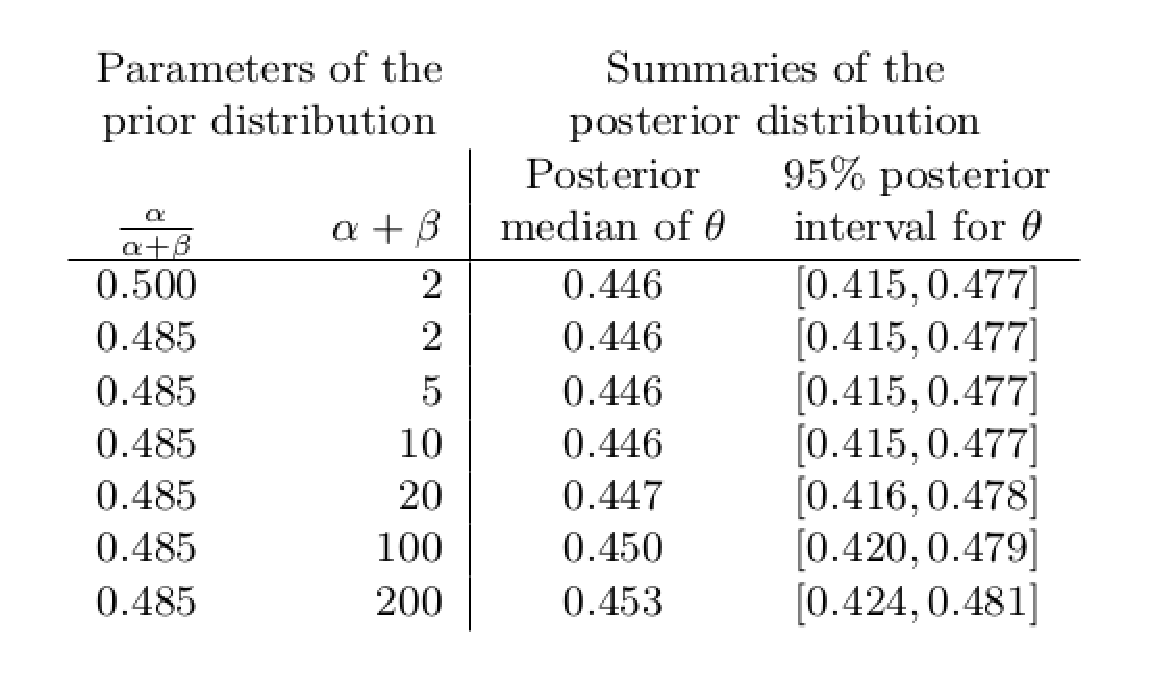
\includegraphics[scale = 0.50]{pictures/tbl_2_1.eps}
\caption{Souhrnné statistiky aposteriorního rozdělení parametru $\theta$; pravděpodobnost narození jedince ženského pohlaví v případě placenta previa pro různá konjugátní apriorní rozdělení}
\label{tbl_2_1}
\end{figure}

První řádek tabulky odpovídá apriornímu rozdělení s parametry $\alpha = 1$ a $\beta = 1$. Následující řádky pak reprezentují apriorní rozdělení, která jsou více a více koncentrovaná okolo hodnoty 0.485. První sloupec představuje apriorní hodnotu parametru $\theta$, druhý sloupec představuje objem apriorní informace vyjádřené jako $\alpha + \beta$.\footnote{Připomeňme si, že $\alpha + \beta - 2$ lze v jistém slova smyslu chápat jako počet apriorních pozorování.} Tabulka také ilustruje skutečnost, že aposteriorní inference založené na velkém počtu pozorování jsou na volbu apriorního rozdělení citlivé jen v omezené míře. Pouze pro spodní řádky tabulky, kdy objem apriorní informace odpovídá 100 až 200 porodů, je aposteriorní rozdělení vychýlenější směrem k apriornímu rozdělení a i tomto případě 95\% konfidenční interval stále nezahrnuje apriorní střední hodnotu.

\subsubsection{Nekonjugátní apriorní rozdělení}

Jako alternativu ke konjugátní rodině beta rozdělení můžeme uvažovat apriorní rozdělení, které je koncentrované okolo hodnoty 0.485 a směrem k chvostům se zplošťuje. Jedním z příkladů takovéhoto rozdělení je rozdělení na obrázku 2.3a. Tato apriorní rozdělení má střední hodnotu 0.493 a směrodatnou odchylku 0.21, což je podobné jako v případě beta rozdělení s parametry $\alpha + \beta = 5$. Nenormalizované aposteriorní rozdělení je možné získat pomocí mřížky $(0.000, 0.001, ..., 1.000)$ pro hodnoty parametru $\theta$ tak, že vynásobíme apriorní hustotu pravděpodobnosti s binomickou věrohodnostní funkcí pro každý bod mřížky. Aposteriorní simulace je pak možné získat normalizací rozdělení nad mřížkou uvažovaných hodnot parametru $\theta$. Obrázek 2.3b představuje histogram 1,000 náhodných výběrů z této aposteriorní pravděpodobnostní funkce. Aposteriorní střední hodnota je 0.448 a 95\% konfidenční interval je $[0.419, 0.480]$. Protože je apriorní pravděpodobnostní funkce přebita aposteriorními pozorováními, odpovídají tyto výsledky výsledkům z tabulky na obrázku 2.2.

\begin{figure}[htp]
\centering
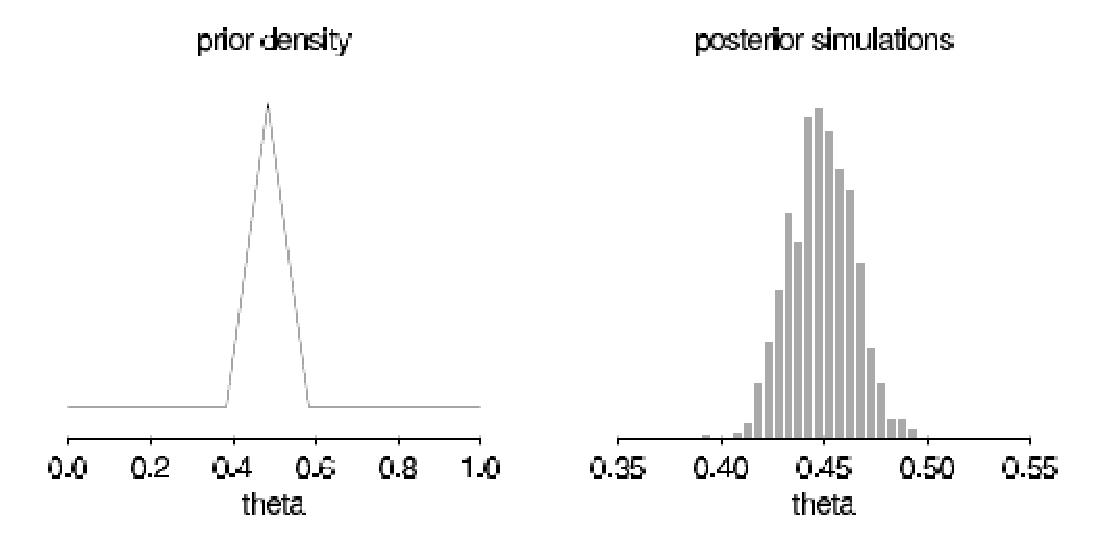
\includegraphics[scale = 0.50]{pictures/fig_2_4.eps}
\caption{(a) apriorní hustota pravděpodobnosti parametru $\theta$ v ilustrativním příkladě nekonjugátní analýzy; (b) histogram 1,000 náhodných výběrů z diskrétní aproximace aposteriorní hustoty pravděpodobnosti}
\label{fig_2_4}
\end{figure}

\section{Odhad normální střední hodnoty při známém rozptylu}

Pomocí centrální limitní věty lze ospravedlnit aplikaci normální věrohodností funkce v situacích, kdy je použití teoreticky správnější věrohodnostní funkce z analytického pohledu problematické. Nicméně v následující kapitole budeme předpokládat, že je použití normálního rozdělení nejen žádoucí ale také vhodné.

Nejprve odvodíme výsledek pro jedno aposteriorní normálně rozdělené pozorování. Na závěr pak tento výsledek zobecníme pro vícero aposteriorních normálně rozdělených pozorování.

\subsection{Jedno aposteriorní pozorování}

\subsubsection{Věrohodnostní funkce}

Uvažujme pozorování $y$ náhodně vybrané z normální rozdělení se střední hodnotou $\theta$ a známým rozptylem $\sigma^2$. Výběrové rozdělení má tvar
\begin{equation}
p(y|\theta) = \frac{1}{\sqrt{2 \pi} \sigma} e^{-\frac{1}{2 \sigma^2}}(y - \theta)^2.
\end{equation}

\subsubsection{Konjugátní apriorní a aposteriorní rozdělení}

Jestliže je věrohodnostní funkce exponenciála kvadratické formy v parametru $\theta$, pak má rodina konjugátních apriorních rozdělení podobu
\begin{equation}
p(\theta) = e^{A \theta^2 + B \theta + C}.
\end{equation}
Tuto rodinu apriorních rozdělení parametrizujeme jako
\begin{equation}
p(\theta) \varpropto e^{-\frac{1}{2 \tau_0^2} (\theta - \mu_0)^2}
\end{equation}
s hyperparametry $\mu_0$ a $\tau_0^2$, tj. $\theta \sim N(\mu_0, \tau_0^2)$. Pro zjednodušení předpokládejme, že známe jak $\mu_0$ tak $\tau_0^2$.

Zvolené apriorní rozdělení implikuje, že aposteriorní rozdělení parametru $\theta$ je rovněž exponenciála kvadratické formy a tudíž se  jedná o normální rozdělení.\footnote{Nicméně může být zapotřebí `trocha' algebry, abychom zjistili její konkrétní podobu.} V případě aposteriorních rozdělení mají všechny parametry s výjimkou $\theta$ charakter konstanty, což vede k podmíněné hustotě pravděpodobnosti
\begin{equation}
p(\theta | y) \varpropto e^{-\frac{1}{2}\Big(\frac{(y  \theta)^2}{\sigma^2} + \frac{(\theta - \mu_0)^2}{\tau_0^2} \Big)},
\end{equation}
kterou lze dále upravit do tvaru
\begin{equation}
p(\theta | y) \varpropto e^{-\frac{1}{2 \tau_1^2}(\tau - \mu_1)^2},
\end{equation}
tj. $\theta | y \sim N(\mu_1, \tau_1^2)$, kde
\begin{equation}
\mu_1 = \frac{\frac{1}{\tau_0^2} \mu_0 + \frac{1}{\sigma^2}y}{\frac{1}{\tau_0^2} + \frac{1}{\sigma^2}}
\end{equation}
a
\begin{equation}
\frac{1}{\tau_1^2} = \frac{1}{\tau_0^2} + \frac{1}{\sigma^2}.
\end{equation}

\subsubsection{Normální rozdělení a přesnost}

Při práci s normálním rozdělením hraje prominentní úlohu inverze rozptylu, kterou označujeme jako přesnost (precision). Rovnice (2.27) ilustruje, že v případě pozorování, které sledují normální rozdělení, a apriorního normálního rozdělení, je aposteriorní přesnost rovna součtu apriorní přesnosti a přesnosti pozorovaných dat.

Existuje několik způsobů, jak interpretovat aposteriorní střední hodnotu $\mu_1$. V (2.26) je aposteriorní střední hodnota vyjádřena jako průměr apriorní střední hodnoty a střední hodnoty pozorování $y$ s použitím vah, které jsou proporcionální přesnostem $1/\tau_0^2$ a $1 / \sigma^2$. Alternativně lze vyjádřit $\mu_1$ jako apriorní střední hodnotu upravenou o pozorování $y$, tj. jako
\begin{equation}
\mu_1 = \mu_0 + (y - \mu_0) \frac{\tau_0^2}{\sigma^2 + \tau_0^2}
\end{equation}
nebo také jako pozorování $y$ vychýlená směrem k apriorní střední hodnotě, tj. jako
\begin{equation}
\mu_1 = y - (y - \mu_0) \frac{\sigma^2}{\sigma^2 + \tau_0^2}.
\end{equation}
Všechny tři výše uvedené interpretace aposteriorní střední hodnoty lze chápat jako kompromis mezi apriorní střední hodnotou a pozorovanými daty.

\subsubsection{Aposteriorní prediktivní rozdělení}

Aposteriorní prediktivní rozdělení lze vyjádřit pomocí integrace (1.5) jako
\begin{equation}
\begin{split}
p(\tilde{y}|y) & = \int p(\tilde{y}|\theta) p(\theta | y) d \theta\\
 & \propto \int e^{-\frac{1}{2 \sigma^2}(\tilde{y} - \theta)^2}e^{-\frac{1}{2 \tau_1^2}(\theta - \mu_1)^2}d\theta.
\end{split}
\end{equation}
První řádek výše uvedené rovnice je platný, protože budoucí pozorování $\tilde{y}$ pro dané $\theta$ nezávisí na minulých pozorováních $y$. Pravděpodobnostní rozdělení $\tilde{y}$ můžeme jednodušeji určit s využitím vlastností dvourozměrného normálního rozdělení. Součin v integrálu druhého řádku je exponenciála kvadratické formy $(\tilde{y}, \theta)$. $\tilde{y}$ a $\theta$ tak sledují aposteriorní sdružené normální rozdělení, což znamená, že marginální aposteriorní rozdělení $\tilde{y}$ je také normální.

S využitím znalosti aposteriorního rozdělení, pro které platí $E(\tilde{y} | \theta) = \theta$ a $var(\tilde{y} | \tilde) = \sigma^2$, společně s (2.7) a (2.8) lze odvodit aposteriorní střední hodnotu
\begin{equation}
E(\tilde{y} | y) = E(E(\tilde{y} | \theta, y) | y) = E(\theta | y) = \mu_1
\end{equation}
a aposteriorní rozptyl
\begin{equation}
\begin{split}
var(\tilde{y} | y) & = E(var(\tilde{y | \theta, y}) | y ) + var(E(\tilde{y} | \theta, y) | y)\\
 & = E(\sigma^2 | y ) + var(\theta | y)\\
 & = \sigma^2 + \tau_1^2.
\end{split}
\end{equation}
Jinými slovy, aposteriorní prediktivní rozdělení $\tilde{y}$ charakterizováno (a) střední hodnotou, která je rovna aposteriorní střední hodnotě $\theta$ a (b) rozptylem, který se skládá prediktivního rozptylu $\sigma^2$ a rozptylu $\tau_1^2$ z titulu aposteriorní nejistoty parametru $\theta$.

\subsection{Vícero aposteriorních pozorování}

V předchozím textu jsme se zabývali situací, kdy jsou aposteriorní data reprezentována jedním pozorováním. Nyní uvažujme realističtější situaci, kdy jsou aposteriorní data reprezentována vícero pozorováními $y = (y_1, ..., y_n)$. Aposteriorní hustota pravděpodobnosti je pak definována jako
\begin{equation}
\begin{split}
p(\theta | y) & \varpropto p(\theta) p(y | \theta)\\
 & = p(\theta) \prod_{i = 1}^n p(y_i | \theta)\\
 & \varpropto e^{-\frac{1}{2 \tau_0^2}(\theta - \mu_0)^2}\prod_{i = 1}^n e^{-\frac{1}{2 \sigma^2}(y_i - \theta)^2}\\
 & \varpropto e^{-\frac{1}{2}\Big(\frac{1}{\tau_0^2}(\theta - \mu_0)^2 + \frac{1}{\sigma^2} \sum_{i = 1}^n (y_i - \theta) ^ 2\Big)}
\end{split}
\end{equation}
Zjednodušením výše uvedeného vztahu lze dokázat, že aposteriorní rozdělení závisí na $y$ pouze skrze výběrový průměr $\overline{y} = \frac{1}{n}\sum_i y_i$, tj. $\overline{y}$ je dostatečná statistika. Protože platí $\overline{y} | \theta, \sigma^2 \sim N(\theta, \sigma^2 / n)$, lze závěry pro jedno pozorování přímo aplikovat také na vícero pozorování, tj.
\begin{equation}
p(\theta | y_1, ..., y_n) = p(\theta | \overline{y}) = N(\theta | \mu_n, \tau_n^2),
\end{equation}
kde
\begin{equation}
\mu_n = \frac{\frac{1}{\tau_0^2}\mu_0 + \frac{n}{\sigma^2}\overline{y}}{\frac{1}{\tau_0^2 + \frac{n}{\sigma^2}}}
\end{equation}
a
\begin{equation}
\frac{1}{\tau_0^2} = \frac{1}{\tau_0^2} + \frac{n}{\sigma^2}.
\end{equation}
Stejný výsledek lze získat také tak, že budeme aposteriorní rozdělení postupně aktualizovat o pozorování $y_1, ..., y_n$.

Rovnice (2.36) nám říká, že pokud $\tau_0 \rightarrow \infty$ pro fixní $n$ nebo $n \rightarrow \infty$ pro fixní $\tau_0^2$, pak
\begin{equation}
p(\theta | y) \approx N(\theta | \overline{y}, \sigma^2 / n),
\end{equation}
což je praxi vhodná aproximace bez ohledu na apriorní rozdělení.

\section{Ostatní jednoparametrové modely}

V praxi obecně neplatí, že aposteriorní rozdělení $p(\theta | y)$ musí mít vždy analytickou formu. Příčinou bývá normalizační konstanta $p(y)$, která s ohledem na integrál v (1.4) často nemá analytické řešení. Nicméně mnoho formálních analýz se soustředí na situace, pro které je dipozici analytické aposteriorní rozdělení.

Standardní aposteriorní rozdělení, jako jsou binomické, normální, Poissonovo a exponenciální rozdělení, lze odvodit při řešení jednoduchých pravděpodobnostních modelů. Jak jsme již zmínili v předchozím textu, binomické rozdělení lze použít v situacích, kdy se snažíme kvantifikovat frekvenci určitého jevu v populaci. Normální rozdělení pak používáme pro náhodné veličiny, které jsou součtem mnoha nezávislých veličin. Poissonovo resp. exponenciální rozdělení se používají pro modelování počtu událostí resp. pro modelování čekací doby (waiting times).

\subsection{Normální rozdělení se známou střední hodnotou a neznámým rozptylem}

Pro $p(y | \theta, \sigma^2) = N(y | \theta, \sigma^2)$ se známou střední hodnotou $\theta$ a neznámým rozptylem $\sigma^2$ má věrohodnostní funkce vektoru $y = (y_1, ..., y_n)$ podobu
\begin{equation}
\begin{split}
p(y | \sigma^2) & \varpropto \sigma^{-n} e^{-\frac{1}{2 \sigma^2} \sum_{i = 1}^n (y_i - \theta)^2}\\
 & = (\sigma^2)^{-n/2} e^{-\frac{n}{2 \sigma^2}\upsilon},
\end{split}
\end{equation}
kde
\begin{equation}
\upsilon = \frac{1}{n}\sum_{i = 1}^n (y_i - \theta)^2
\end{equation}
je dostatečná statistika.

Odpovídající konjugátní apriorní rozdělení parametru $\sigma^2$ má pak podobu inverzního gamma rozdělení
\begin{equation}
p(\sigma^2) \varpropto (\sigma^2)^{-(\alpha + 1) e^{-\beta / \sigma^2}}
\end{equation}
s hyperparametry $(\alpha, \beta)$. Tento vztah lze však také vyjádřit pomocí inverzního $\chi^2$ rozdělení s parametrem $\sigma_0^2$ a $\nu_0$ stupni volnosti. Jinými slovy, parametr $\sigma^2$ sleduje rozdělení $\sigma_0^2 \nu_0 / X$ kde $X$ je $\chi^2_{\nu_0}$ náhodná veličina; v následujícím textu budeme použít poněkud nestandardní označení $\sigma^2 \sim \textit{Inv-}\chi^2(\nu_0, \sigma_0^2)$.

Výsledné aposteriorní rozdělení parametru $\sigma^2$ má pak tvar
\begin{equation}
\begin{split}
p(\sigma^2 | y) & \varpropto p(\sigma^2)p(y | \sigma^2)\\
 & \varpropto \Big(\frac{\sigma_0^2}{\sigma^2}\Big)^{\frac{\nu_0}{2} + 1} e^{-\frac{\nu_0 \sigma_0^2}{2 \sigma^2}} (\sigma^2)^{-n/2} e^{-\frac{n}{2} \frac{\upsilon}{\sigma^2}}\\
  & \varpropto (\sigma^2) ^ {-\frac{n + \nu_0}{2} + 1}e^{-\frac{1}{2 \sigma^2}(\nu_0 \sigma^2_0 + n \upsilon)}
\end{split}
\end{equation}
nebo-li
\begin{equation}
\sigma^2 | y \sim \textit{Inv-}\chi^2 \Big(\nu_0 + n, \frac{\nu_0 \sigma_0^2 + n \upsilon}{\nu_0 + n} \Big),
\end{equation}
což je inverzní $\chi^2$ rozdělení se škálovacím parametrem $\frac{\nu_0 \sigma_0^2 + n \upsilon}{\nu_0 + n}$ a $\nu_0 + n$ stupni volnosti. Ve světle (2.42) je tak na apriorní rozdělení možné pohlížet jako na aposteriorní rozdělení založené na $\nu_0$ pozorováních s rozptylem $\sigma_0^2$.

\subsection{Poissonův model}

Poissonovo rozdělení se běžně používá v situacích, kdy je předmětem zájmu frekvence určité události v populaci, jako je tomu např. v epidemiologii. Jestliže jedno jednotlivé pozorování $y$ sleduje Poissonovo rozdělení s parametrem $\theta$, pak je jeho pravděpodobnostní rozdělení definováno jako
\begin{equation}
p(y|\theta) = \frac{\theta^y e^{-\theta}}{y!} \textit{ kde } y = 0, 1, ...
\end{equation}
V případě vektoru $y = (y_1, ..., y_n)$ má pak věrohodnostní funkce podobu
\begin{equation}
\begin{split}
p(y | \theta) & = \prod_{i = 1}^n \frac{1}{y_i!} \theta^{y_i} e^{-\theta}\\
 & \varpropto \theta^{t(y)}e^{-n \theta},
\end{split}
\end{equation}
kde $t(y) = \sum_{i = 1}^n y_i$ je dostatečná statistika. Věrohodnostní funkci můžeme přepsat do tvaru rodiny exponenciálních rozdělení jako
\begin{equation}
p(y | \theta) \varpropto e^{-n \theta} e^{t(y) \ln(\theta)}
\end{equation}
s přirozeným parametrem $\phi(\theta) = \ln(\theta)$.

Přirozené konjugátní apriorní rozdělení má podobu
\begin{equation}
p(\theta) \varpropto (e^{-\theta})^{\eta} e^{\nu \ln(\theta)}
\end{equation}
s hyperparametry $(\eta, \nu)$. Jinými slovy, věrohodnostní funkce má tvar $\theta^{\alpha} e^{-b \theta}$, a proto musí mít apriorní pravděpodobnost tvar $p(\theta) \varpropto \theta^A e^{-B \theta}$. Výše uvedenou formu apriorního rozdělení tak lze také vyjádřit jako
\begin{equation}
p(\theta) \varpropto e^{-\beta \theta} \theta^{\alpha - 1},
\end{equation}
což je gamma rozdělení s parametry $\alpha$ a $\beta$. Porovnáním $p(y | \theta)$ a $p(\theta)$ zjistíme, že apriorní rozdělení lze v jistém slova smyslu chápat jako aposteriorní rozdělení založené na $\alpha - 1$ realizacích z celkového počtu $\beta$ pozorování.

Pro výše uvedené apriorní rozdělení má pak aposteriorní rozdělení podobu
\begin{equation}
\theta | y \sim \textit{Gamma}(\alpha + n\overline{y}, \beta + n).
\end{equation}

\subsection{Negativní binomický model}

V případě konjugátních rodin pravděpodobnostních rozdělení lze použít znalost apriorního a aposteriorního rozdělení k odvození marginálního rozdělení $p(y)$ pomocí
\begin{equation}
p(y) = \frac{p(y | \theta) p(\theta)}{p(\theta | y)}.
\end{equation}
Například pro Poissonův model má apriorní prediktivní rozdělení tvar
\begin{equation}
\begin{split}
p(y) & = \frac{\textit{Possion}(y | \theta) \textit{Gamma}(\theta | \alpha, \beta)}{\textit{Gamma}(\theta | \alpha + y, 1 + \beta)}\\
 & = \frac{\Gamma(\alpha + y)\beta^{\alpha}}{\Gamma(\alpha) y! (1 + \beta)^{\alpha + y}},
\end{split}
\end{equation}
což lze dále zredukovat na
\begin{equation}
\begin{split}
p(y) = {{\alpha + y + 1} \choose y} \Big(\frac{\beta}{\beta + 1}\Big)^{\alpha} \Big(\frac{1}{\beta + 1}\Big)^y.
\end{split}
\end{equation}
Tento vztah představuje tzv. negativní binomické rozdělení. V následujícím textu pro něj budeme používat notaci $y \sim \textit{Neg-bin}(\alpha, \beta)$. Výše uvedené odvození ukazuje, že negativní binomické rozdělení je kombinací Poissonových rozdělení s parametry $\theta$, které sledují gamma rozdělení, tj.
\begin{equation}
\textit{Neg-bin}(y | \alpha, \beta) = \int \textit{Poisson}(y | \theta) \textit{Gamma}(\theta | \alpha, \beta) d \theta.
\end{equation}

\subsection{Poissonův model parametrizovaný pomocí míry a expozice}

V řadě praktických situacích je žádoucí rozšířit Poissonův model o pozorování $y_1, ..., y_n$ do podoby
\begin{equation}
y_i \sim \textit{Poisson}(x_i\theta),
\end{equation}
kde $x_i$ jsou známé kladné hodnoty vysvětlující veličiny a $\theta$ je hledaný parametr. V epidemiologii je $\theta$ často nazýván mírou (např. počet úmrtí na 100~000 obyvatel) a $x_i$ expozicí (např. počet obyvatel města). Tento model sice není zaměnitelný z pohledu $y_i$ (tj. záleží na pořadí hodnot $y_i$), nicméně je zaměnitelný z pohledu $(x, y)_i$.

Věrohodnostní funkce v tomto rozšířeném Poissonově modelu má podobu
\begin{equation}
p(y|\theta) \varpropto \theta^{\sum_{i = 1}^n y_i} e^{-(\sum_{i = 1}^n x_i) \theta}
\end{equation}
při ignorování členů, které jsou nezávislé na $\theta$. Pro apriorní rozdělení
\begin{equation}
\theta \sim \textit{Gamma}(\alpha, \beta)
\end{equation}
tak získáváme aposteriorní rozdělení
\begin{equation}
\theta | y \sim \textit{Gamma}\Big(\alpha + \sum_{i = 1}^n y_i, \beta + \sum_{i = 1}^n x_i \Big).
\end{equation}

\subsubsection{Ilustrativní příklad}

Předpokládejme, že ve městě s 200~000 obyvateli zemřeli v minulém roce na astma tři lidé. Na základě této informace můžeme odhadnout míru úmrtnosti v souvislosti s astmatem na 1.50 případů na 100,000 obyvatel. Pro Poissonův model můžeme výběrovou funkci pro $y$ definovat jako $Poisson(2.0 \theta)$, kde $\theta$ představuje skutečnou dlouhodobou míru úmrtnosti na astma. V našem konkrétním případě víme, že $y = 3$ a $x = 2.0$ (protože $\theta$ je vyjádřeno na 100~000 obyvatel), přičemž hledáme hodnotu parametru $\theta$. Pro konstrukci apriorního rozdělení parametru $\theta$ můžeme použít celosvětové statistiky úmrtí na astma a zkombinovat je s informací $y = 3$ s cílem získat aposteriorní rozdělení.

Mortalita v zemích západní Evropy je výrazně nižší než v případě našeho města - cca 0.60 případů na 100~000 obyvatel. V podobných případech je vhodné apriorní rozdělení parametru $\theta$ aproximovat pomocí gamma rozdělení. Jako přijatelný kandidát se jeví $Gamma(3.0, 5.0)$ rozdělení, které má střední hodnotu 0.60 a pro které je 97.50\% všech hodnot menších než 1.44. V praxi při kalibraci hledaného gamma rozdělení zpravidla nejčastěji zafixujeme podíl parametrů v souladu s apriorní střední hodnotou a následně hledáme jejich hodnotu tak, aby výsledné rozdělení splňovalo naše představy konkrétního kvantilu.

Vztah (2.56) nám říká, že aposteriorní rozdělení parametru $\theta$ má při apriorním rozdělením $Gamma(\alpha, \beta)$ tvar $Gamma(\alpha + y, \beta + x)$, což v našem konkrétním případě znamená $Gamma(6.0, 7.0)$. Toto pravděpodobnostní rozdělení má střední hodnotu 0.86, což je v porovnání s napozorovanou frekvencí 1.50 případů na 100~000 obyvatel významně blíže apriorní střední hodnotě 0.60.

Předpokládejme, že namísto jednoho roku máme k dispozici pozorování za deset let, během kterých zemřelo v našem městě 30 lidí. Aposteriorní rozdělení parametru $\theta$ má pak podobu $Gamma(33.0, 25.0)$ a aposteriorní střední hodnotu 1.32, tj. mnohem blíže pozorované úmrtnosti.

\subsection{Exponenciální model}

Exponenciální rozdělení je běžně používáno pro modelování doby, která uplyne mezi dvěma událostmi, tzv. čekací doby. Výběrové rozdělení $y$ pro daný parametr $\theta$ má tvar
\begin{equation}
p(y|\theta) = \theta e^{-y \theta} \textit{ pro } y > 0,
\end{equation}
kde $\theta = 1 / E(y | \theta)$ nazýváme mírou. Matematicky je exponenciální rozdělení speciálním případem gamma rozdělení s parametry $(\alpha, \beta) = (1, \theta)$.

Exponenciální rozdělení je bez paměti, což z něj činí přirozenou volbu pro modelování přežití resp. dožití. Lze ho použít např. v situaci, kdy pravděpodobnost, že daný subjekt přežije dodatečný čas v délce $t$, je nezávislá na čase $s$, který již uplynul, tj. $Pr(y > t + s | y > s, \theta) = Pr(y > t | \theta)$ pro libovolné $s$ a $t$. Konjugátní apriorní rozdělení pro exponenciální parametr $\theta$ je (stejně jako pro Poissonovo rozdělení) $\textit{Gamma}(\theta | \alpha, \beta)$ s odpovídajícím aposteriorním rozdělením $\textit{Gamma}(\theta | \alpha + 1, \beta + y)$. Výběrové rozdělení $n$ nezávislých pozorování $y = (y_1, ..., y_n)$ s konstantní mírou $\theta$ má tvar
\begin{equation}
p(y | \theta) = \theta^n e^{-n \overline{y} \theta} \textit{ pro } \overline{y} \ge 0,
\end{equation}
a je, pokud ho chápeme jako věrohodnostní funkci parametru $\theta$ pro fixní $y$, proporcionální $Gamma(n + 1, n \overline{y})$ rozdělení. Proto je možné na apriorní rozdělení $Gamma(\alpha, \beta)$ parametru $\theta$ pohlížet jako na $\alpha - 1$ exponenciálních rozdělení s celkovou čekací dobou $\beta$.

\section{Ilustrativní příklad - rakovina ledvin v USA}

\subsection{Rozložení případů napříč USA}

Následující mapa USA zobrazuje okresy s nejvyšší mírou úmrtí na rakovinu ledvin v průběhu let 1980 - 1989. Z mapy se zdá, že mezi nejvíce postižené okresy patří ty z oblasti Velkých plání. Pokud bychom však měli k dispozici podrobnější informace, zjistili bychom, že se na Velkých plání současně nachází také okresy s nejnižší mírou úmrtí. Důvodem tohoto zdánlivého paradoxu je velikost okresů. Uvažujme okres s 1~000 obyvatel. Rakovina ledvin je poměrně vzácné onemocnění, a tak se může snadno stát, že v průběhu deseti let nikdo nezemře a okres bude vykazovat nulovou míru úmrtnosti. Naopak, pokud zemře jeden člověk, bude okres vykazovat míru úmrtnosti 1 na 10~000 člověkoroků, což je dostatečné na to, aby figuroval na výše zmiňované mapě. A právě Velké pláně jsou charakteristické velkým počtem okresů s nízkým počtem obyvatel.

\begin{figure}[htp]
\centering
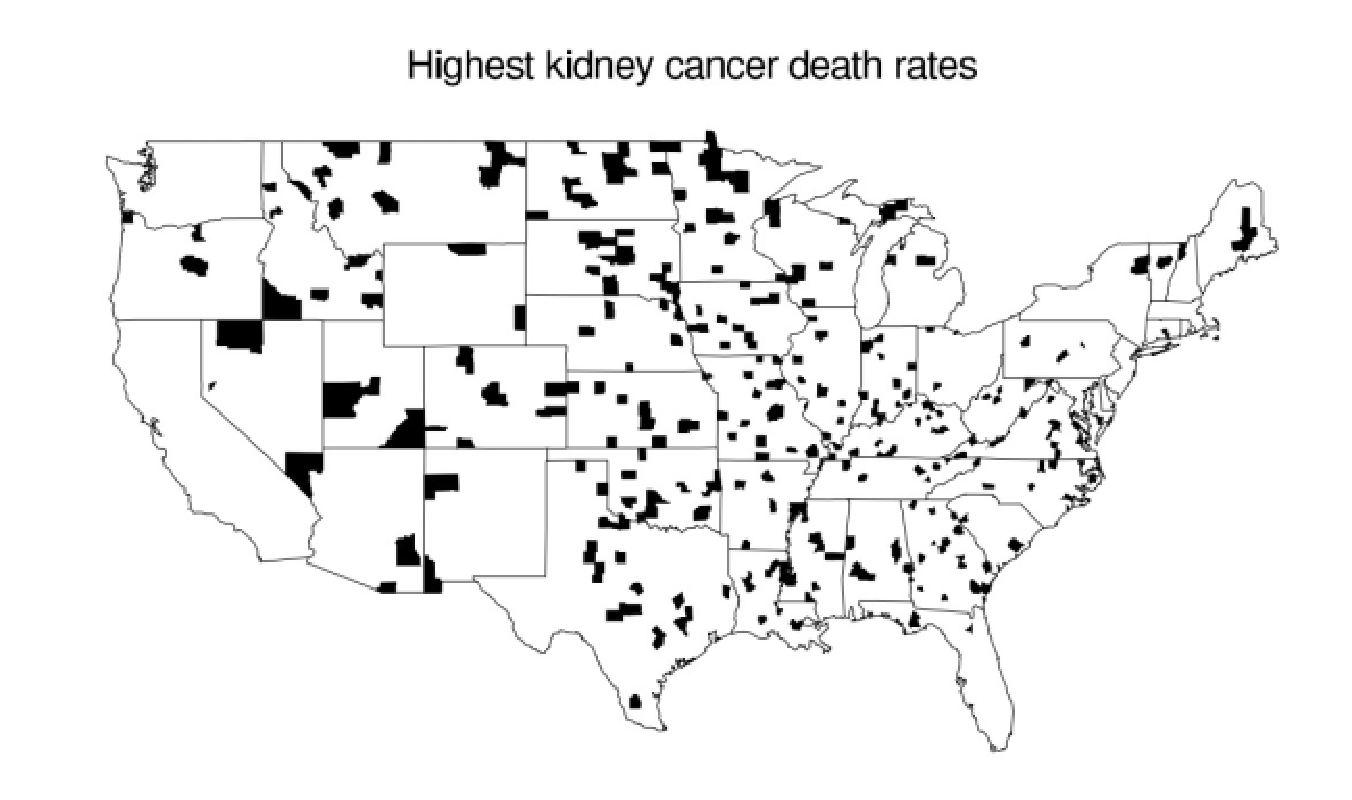
\includegraphics[scale = 0.50]{pictures/fig_2_6.eps}
\caption{Okresy v USA s nejvyšší mírou úmrtnosti na rakovinu ledvin v průběhu let 1980 - 1989}
\label{fig_2_6}
\end{figure}

\subsection{Bayesiánská inference}

Paradox Velkých plání indikuje, že je pro jednotlivé okresy vhodné použít model
\begin{equation}
y_i \sim Poisson(10 \cdot n_j \theta_j),
\end{equation}
kde $y_j$ je počet úmrtí na rakovinu ledvin v rámci okresu $j$, $n_j$ je počet obyvatel okresu, a $\theta_j$ je míra úmrtnosti přepočtena na osobu a rok. Zásadní rozdíl oproti (2.53) je ten, že míra úmrtnosti je specifická pro každý okres, tj. $\theta_j$ je odhadováno separátně pro každý okres.

Pro účely Bayesiánské inference potřebuje definovat apriorní rozdělení neznámého parametru $\theta_j$. Pro tyto účely použijeme gamma rozdělení $Gamma(20, 430~000)$, které konjuguje do Poissonova rozdělení. Apriorní rozdělení má střední hodnotu $\frac{\alpha}{\beta} = 4.65 \cdot 10^{-5}$ a směrodatnou odchylku $\frac{\sqrt{\alpha}}{\beta} = 1.04 \cdot 10^{-5}$.

Aposteriorní rozdělení má pak podobu
\begin{equation}
\theta_j | y_j \sim \textit{Gamma}(20 + y_j, 430~000 + 10n_j)
\end{equation}
se střední hodnotou
\begin{equation}
E(\theta_j | y_j) = \frac{20 + y_j}{430~000 + 10 n_j}
\end{equation}
a rozptylem
\begin{equation}
var(\theta_j | y_j) = \frac{20 + y_j}{(430~000 + 10 n_j)^2}.
\end{equation}
Aposteriorní střední hodnotu je možné chápat jako vážený průměr pozorované míry úmrtnosti $\frac{y_j}{10 n_j}$ a apriorní střední hodnoty $\frac{\alpha}{\beta} = 4.65 \cdot 10^{-5}$.

\subsection{Důsledky velikosti okresu}

Relativní váha apriorní informace se odvíjí od velikosti populace $n_j$. Pro ilustraci uvažujme okres s $n_j = 1~000$ obyvateli.
\begin{itemize}
\item Jestliže $y_j = 0$, pak se pozorovaná míra úmrtnosti rovná nule, avšak aposteriorní střední hodnota je $\frac{20}{440~000} = 4.55 \cdot 10^{-5}$.
\item Jestliže $y_j = 1$, je pozorovaná míra úmrtnosti rovna $1.00 \cdot 10^{-4}$, nicméně aposteriorní střední hodnota je pouze $\frac{21}{440~000} = 4.77 \cdot 10^{-5}$.
\item Jestliže $y_j = 2$, je pozorovaná míra úmrtnosti rovna $2.00 \cdot 10^{-4}$, ale aposteriorní střední hodnota je stále $\frac{21}{440~000} = 4.77 \cdot 10^{-5}$.
\end{itemize}
Je tedy zřejmé, že pro okres s malým počtem obyvatel je aposteriorní rozdělení do značné míry definováno apriorním rozdělením. V případě okresu, který má např. 1~000~000 obyvatel by tomu bylo opačně.

V Poissonově modelu (2.59) je rozptyl pozorované úmrtnosti $\frac{y_j}{10 \cdot n_j}$ inverzní k expozičnímu parametru $n_j$. Jinými slovy, okresy s malým počtem obyvatel vykazují vyšší míru fluktuace v úmrtnosti. To vysvětluje, proč okresy s malým počtem obyvatel patří současně mezi okresy s malou i velkou mírou úmrtí na rakovinu ledvin.

\section{Neinformativní apriorní rozdělení}

V případě, že je apriorní rozdělení spíše než na datech založeno na expertním odhadu, nazýváme toto apriorní rozdělení neinformativním. Vzhledem k značné nejistotě neinformativního apriorního rozdělení je přirozená snaha o minimalizaci jeho vlivu na aposteriorní rozdělení.

Kromě neinformativního apriorního rozdělení rozeznáváme také slabě informativní apriorní rozdělení zohledňující určitou omezenou informaci, která je např. dostatečná na to, aby vytyčila rozumné rozmezí hodnot hledaného parametru.

\subsection{Vlastní na nevlastní apriorní rozdělení}

Vraťme se k problematice odhadu střední hodnoty $\theta$ v rámci normálního modelu se známým rozptylem $\sigma^2$ a apriorním rozdělením $N(\mu_0, \tau_0^2)$ parametru $\theta$. Jestliže je apriorní přesnost $1 / \tau_0^2$ v porovnání s datovou přesností $n / \sigma^2$ malá, pak je aposteriorní rozdělení přibližně stejné jako v případě $\tau_0^2 = \infty$, tj.
\begin{equation}
p(\theta | y) \approx N(\theta | \overline{y}, \sigma^2 / n).
\end{equation}
Aposteriorní rozdělení je tak přibližně rovno rozdělení, které bychom získali za předpokladu, že $p(\theta)$ je proporcionální konstantě pro $\theta \in (-\infty, \infty)$. Takovéto rozdělení však není možné, protože integrál přes uvažované $p(\theta)$ by nebyl konečný, což je v rozporu s předpokladem, že součet pravděpodobností je roven jedné. Obecně nazýváme apriorní rozdělení $p(\theta)$ vlastním (proper), pokud je nezávislé na pozorovaných datech a jeho integrál je roven jedné.\footnote{Pokud je integrál $p(\theta)$ konečný a větší než jedna, nazýváme $p(\theta)$ nenormalizovaným rozdělením. Vynásobením vhodnou konstantou je možné $p(\theta)$ znormalizovat tak, aby byl integrál roven jedné.} Ačkoliv je apriorní rozdělení uvedené v tomto případě nevlastní (improper), aposteriorní rozdělení je vlastní.

Jako druhý příklad neinformativního apriorního rozdělení uvažujme normální model se známou střední hodnotou a neznámým rozptylem s apriorním inverzním $\chi^2$ rozdělením. Jestliže je apriorní počet stupňů volnosti $\nu_0$ v porovnání se stupni volnosti dat $n$ malý, pak je aposteriorní rozdělení přibližně stejné jako v případě $\nu_0 = 0$, tj.
\begin{equation}
p(\sigma^2 | y) \approx \textit{Inv-}\chi^2(\sigma^2 | n, \upsilon).
\end{equation}
K této limitní formě aposteriorního rozdělení lze také dojít tak, že apriorní rozdělení parametru $\sigma^2$ definujeme jako $p(\sigma^2) \varpropto 1 / \sigma^2$. Protože je jeho integrál nad intervalem $(0, \infty)$ nekonečný, je toto rozdělení nevlastním rozdělením.

\subsection{Nevlastní apriorní vs. vlastní aposteriorní rozdělení}

Definujme nenormalizované aposteriorní rozdělení
\begin{equation}
p(\theta | y) \varpropto p(y | \theta) p(\theta).
\end{equation}
Ve výše uvedených příkladech je aposteriorní rozdělení vlastní, tj. $\int p(\theta | y) d \theta$ je konečné pro všechna $y$. To však nemusí vždy platit. Při interpretaci aposteriorního rozdělení založeného na nevlastním apriorním rozdělením je třeba zvýšené opatrnosti. Je nutné zkontrolovat, že aposteriorní rozdělení má konečný integrál a smysluplnou formu. Takto získané aposteriorní rozdělení pak lze interpretovat jako aproximaci v případech, kdy kontribuce věrohodnostní funkce dominuje nad apriorním rozdělením.

\subsection{Jeffreyovo pravidlo}

Uvažujme transformaci $\phi = h(\theta)$, která každé hodnotě $\theta$ přiřadí právě jednu hodnotu $\phi$. Apriorní rozdělení $p(\theta)$ je tak informačně ekvivalentní apriornímu rozdělení $p(\phi)$, kdy
\begin{equation}
p(\phi) = p(\theta) \begin{vmatrix}\frac{d \theta}{d \phi}\end{vmatrix} = p(\theta) | h'(\theta)|^{-1}.
\end{equation}
Jakékoliv pravidlo, které určuje apriorní rozdělení $p(\theta)$, by tak mělo vést k ekvivalentnímu výsledku, pokud je aplikované na transformovaný parametr $h(\theta)$. Jinými slovy, $p(\phi)$ vypočtené na základě (2.66) by mělo odpovídat $p(\phi)$ získanému přímo pomocí transformačního modelu $p(y, \phi) = p(\phi)p(y | \phi)$.

Jeffreyovo pravidlo tak umožňuje definovat neinformativní apriorní rozdělení jako $p(\theta) \varpropto |J(\theta)|^{1/2}$, kde $J(\theta)$ je tzv. Fisherova informace pro parametr $\theta$, tj.
\begin{equation}
J(\theta) = E\Big(\Big(\frac{d \ln(p(y | \theta))}{d \theta}\Big)^2 | \theta \Big) = - E\Big(\frac{d^2 \ln(p(y | \theta))}{d \theta^2} | \theta \Big).
\end{equation}
Abychom se přesvědčili, že je Jeffreyův apriorní model invariantní, stačí $J(\phi)$ vyjádřit v bodě $\theta = h^{-1}(\phi)$, tj.
\begin{equation}
\begin{split}
J(\phi) & =  - E\Big(\frac{d^2 \ln(p(y|\phi))}{d \phi^2}\Big)\\
 & = - E\Big({d^2 \ln \big(p(y|\theta = h^{-1}(\phi))\big)}\begin{vmatrix}\frac{d \theta}{d \phi}\end{vmatrix}^2\Big)\\
 & = J(\theta)\begin{vmatrix}\frac{d \theta}{d \phi}\end{vmatrix}^2,
\end{split}
\end{equation}
a proto $J(\phi)^{1/2} = J(\theta)\begin{vmatrix}\frac{d \theta}{d \phi}\end{vmatrix}$.

\subsection{Neinformativní apriorní rozdělení pro binomický parametr}

Uvažujme binomické rozdělení $y \sim \textit{Bin}(n, \theta)$, která má logaritmickou věrohodnostní funkci
\begin{equation}
\ln p(y | \theta) = \textit{konstanta } + y \ln(\theta) + (n - y)\ln(1 - \theta).
\end{equation}
Aplikací druhé derivace a substitucí $E(y | \theta) = n \theta$ získáváme Fisherovu informaci
\begin{equation}
J(\theta) = - E \Big(\frac{d^2 \ln(p(y | \theta))}{d \theta ^ 2} | \theta \Big) = \frac{n}{\theta(1 - \theta)}.
\end{equation}
Nenormalizované apriorní rozdělení je pak $p(\theta) \varpropto \theta^{-1/2}(1 - \theta)^{-1/2}$, což je $\textit{Beta}(\frac{1}{2}, \frac{1}{2})$ rozdělení.

\subsection{Klíčová hodnota, lokační a škálovací parametr}

Pro binomický model a jiné jednoparametrové modely vede aplikace rozdílných principů k rozdílným neinformativním apriorním rozdělením. Nicméně ve dvou případech - lokačních a škálovacích parametrech - se všechny principy shodují.
\begin{enumerate}
\item Jestliže je pravděpodobnostní funkce veličiny $y$ taková, že $p(y - \theta | \theta)$ je funkce, která neobsahuje $\theta$ a $y$ jako separátní proměnné - řekněme $f(u)$, kde $u = y - \theta$ - pak je $(y - \theta)$ tzv. klíčová hodnota (pivotal quantity) a $\theta$ lokační parametr (location parameter). V takovém případě je žádoucí, aby neinformativní apriorní rozdělení parametru $\theta$ implikovalo $f(y - \theta)$ pro aposteriorní rozdělení $p(y - \theta | y)$. To znamená, že i pro aposteriorní rozdělení by $(y - \theta)$ měla být klíčovou hodnotnou, a nemělo by tak neobsahovat $\theta$ ani $y$ jako separátní proměnné. S použitím Bayesovy věty $p(y - \theta | y) \varpropto p(\theta)p(y - \theta | \theta)$ tato podmínka znamená, že neinformativní apriorní rozdělení je uniformní v $\theta$, tj. $p(\theta) \varpropto \textit{ konstanta}$ nad intervalem $(-\infty, \infty)$.
\item Jestliže je pravděpodobnostní funkce veličiny $y$ taková, že $p(\frac{y}{\theta} | \theta)$ je funkce, která neobsahuje $\theta$ a $y$ jako separátní proměnné - řekněme $f(u)$, kde $u = \frac{y}{\theta}$ - pak je $\frac{y}{\theta}$ klíčová hodnota a $\theta$ škálovací parametr (scale parametr). V takovém případě je žádoucí, aby neinformativní apriorní rozdělení parametru $\theta$ implikovalo $f(\frac{y}{\theta})$ pro aposteriorní rozdělení $p(\frac{y}{\theta} | y)$. Transformací proměnných lze podmíněnou pravděpodobnost $y$ pro dané $\theta$ lze vyjádřit pomocí podmíněné pravděpodobnosti $u$ pro dané $\theta$ jako
\begin{equation}
p(y | \theta) = \frac{1}{\theta} p(u | \theta)
\end{equation}
a podobně
\begin{equation}
p(\theta | y) = \frac{y}{\theta^2}p(u | \theta).
\end{equation}
Předpokladem $p(u | \theta) = p(u | y) = g(u)$ se pak dostáváme k identitě $p(\theta | y) = \frac{y}{\theta}p(y | \theta)$. To implikuje apriorní rozdělení $p(\theta) \varpropto \frac{1}{\theta}$ popř. ekvivalentně $p(\ln(\theta)) \varpropto 1$ nebo $p(\theta^2) \varpropto \frac{1}{\theta ^ 2}$.
\end{enumerate}

\subsection{Komplikace spojené s neinformativním apriorním rozdělením}

\begin{enumerate}
\item Hledání univerzálního apriorního rozdělení je zavádějící. Jestliže věrohodnostní funkce dominuje, není volba relativně `plochého' apriorního rozdělení na škodu. Nicméně volba určitého apriorního rozdělení jako reference vede často k jeho automatické aplikaci i v situacích, kdy to není žádoucí.
\item V řadě praktických problémů neexistuje zřejmá volba pro vágní apriorní rozdělení, protože pravděpodobnostní rozdělení, které je `ploché' nebo uniformní pro jednu parametrizaci, nemusí být `ploché' nebo uniformní pro jinou parametrizaci. Například rozumné apriorní rozdělení střední hodnoty $\theta$ je uniformní, zatímco v případě $\sigma^2$ se jako rozumné apriorní rozdělení zdá $p(\sigma^2) \varpropto 1 / \sigma^2$. Nicméně pokud definujeme transformaci $\phi = \ln(\sigma^2)$, pak má apriorní rozdělení parametru $\phi$ tvar
\begin{equation}
p(\phi) = p(\sigma^2) \begin{vmatrix}\frac{d \sigma^2}{d \phi}\end{vmatrix} \varpropto \frac{1}{\sigma^2} \sigma^2 = 1,
\end{equation}
tj. je uniformní pro $\phi = \ln(\sigma^2)$.
\item Další komplikace se objevují při průměrování několika alternativních modelů, které zahrnují nevlastní apriorní rozdělení. Touto problematikou se budeme zabývat v kapitole 7.
\end{enumerate}

Navzdory výše uvedeným problémům jsou neinformativní apriorní rozdělení užitečná pokud (a) je nalezení skutečného apriorního rozdělení komplikované nebo nemožné a (b) jsme ochotni zkontrolovat smysluplnost výsledného aposteriorního rozdělení a to, že se jedná o funkci vlastní.

\section{Slabě informativní apriorní rozdělení}

Apriorní rozdělení označujeme jako slabě informativní, pokud se jedná o vlastní rozdělení, které je zkonstruováno tak, že vědomě zohledňuje slabší informaci, než jaká je k dispozici. V praxi často namísto úplné informační rezignace zkonstruujeme apriorní rozdělení, které je při relativně omezené informační hodnotě stále smysluplné. Klasickým příkladem je apriorní rozdělení poměru novorozenců ženského pohlaví v populaci. Neinformativní apriorní rozdělení může být založené na uniformním rozdělení nad intervalem $[0.00, 1.00]$; slabě informativní apriorní rozdělení by pak tento interval omezilo na $[0.40, 0.60]$. V řadě případů ani není možné popř. praktické do apriorního rozdělení zahrnout všechnu informaci, kterou máme v době konstrukce modelu k dispozici.

Slabě informativní apriorní rozdělení můžeme zkonstruovat dvěma způsoby. Buď začneme s neinformativním apriorním rozdělením, které následně obohatíme o část apriorní informace nebo naopak začneme s informativním apriorním rozdělením, které následně informačně oslabíme
.
